\chapter{Results and Statistical Validation}\label{ch:results}

This chapter presents the retrospective temporal results, their uncertainty,
and the limited external INCART check. Binary detection, conditional subtype
classification, and whole-system classification are reported separately
because they use different sets of beats. All results use the local
window-preparation procedure described in Chapter~\ref{ch:method}.
The saved experiment and prediction files are listed in the appendix.

\section{Evaluation populations and sample sizes}

The final dataset contains 104,755 accepted beats from 46 MITDB MLII records,
representing 45 subject clusters. Records 102 and 104 lack MLII and are excluded.
Records 201 and 202 form one subject cluster. The first and last eligible
beat in each record are excluded because a preceding or following accepted
R peak is unavailable. Compared with the original cache, this removes
92 beats before splitting. Percentages refer to accepted-beat order.

\begin{figure}[H]
\centering
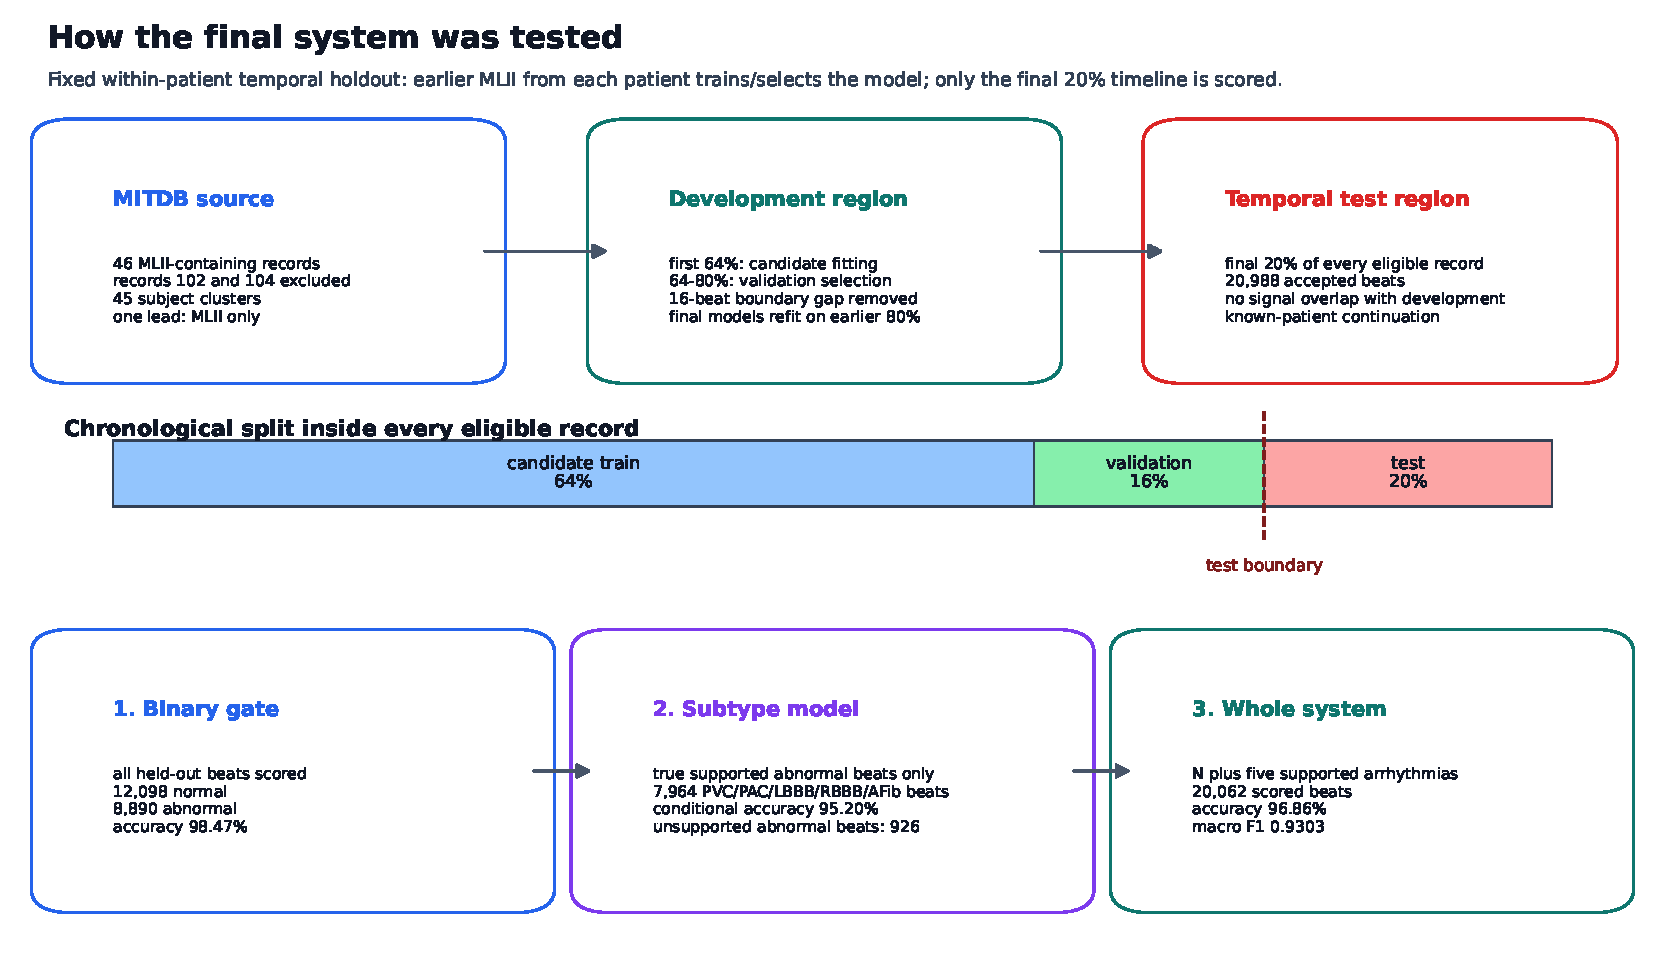
\includegraphics[width=.98\textwidth]{pic/generated/final_testing_protocol.pdf}
\caption[Three evaluation questions and their test populations.]{Evaluation
groups for the corrected retrospective test. Conditional subtype scoring
bypasses the binary gate; complete-system scoring applies the hierarchy.
Counts overlap, and records 201 and 202 share one patient cluster.}
\label{fig:final-testing-protocol}
\end{figure}

\begin{table}[H]
\centering
\caption{Distinct denominators for the three evaluation questions.}
\label{tab:final-test-data}
\begin{tabular}{l>{\raggedright\arraybackslash}p{9cm}}
\toprule
Evaluation & Support and interpretation\\
\midrule
Binary detection & 20,969 beats: 12,085 N and 8,884 abnormal, including
926 unsupported abnormal beats.\\
Conditional subtype & 7,958 true supported abnormal beats, scored by the
subtype model regardless of the binary gate.\\
Whole system & 20,043 beats with supported labels, evaluated through both
stages of the hierarchy.\\
\bottomrule
\end{tabular}
\end{table}

\begin{figure}[H]
\centering
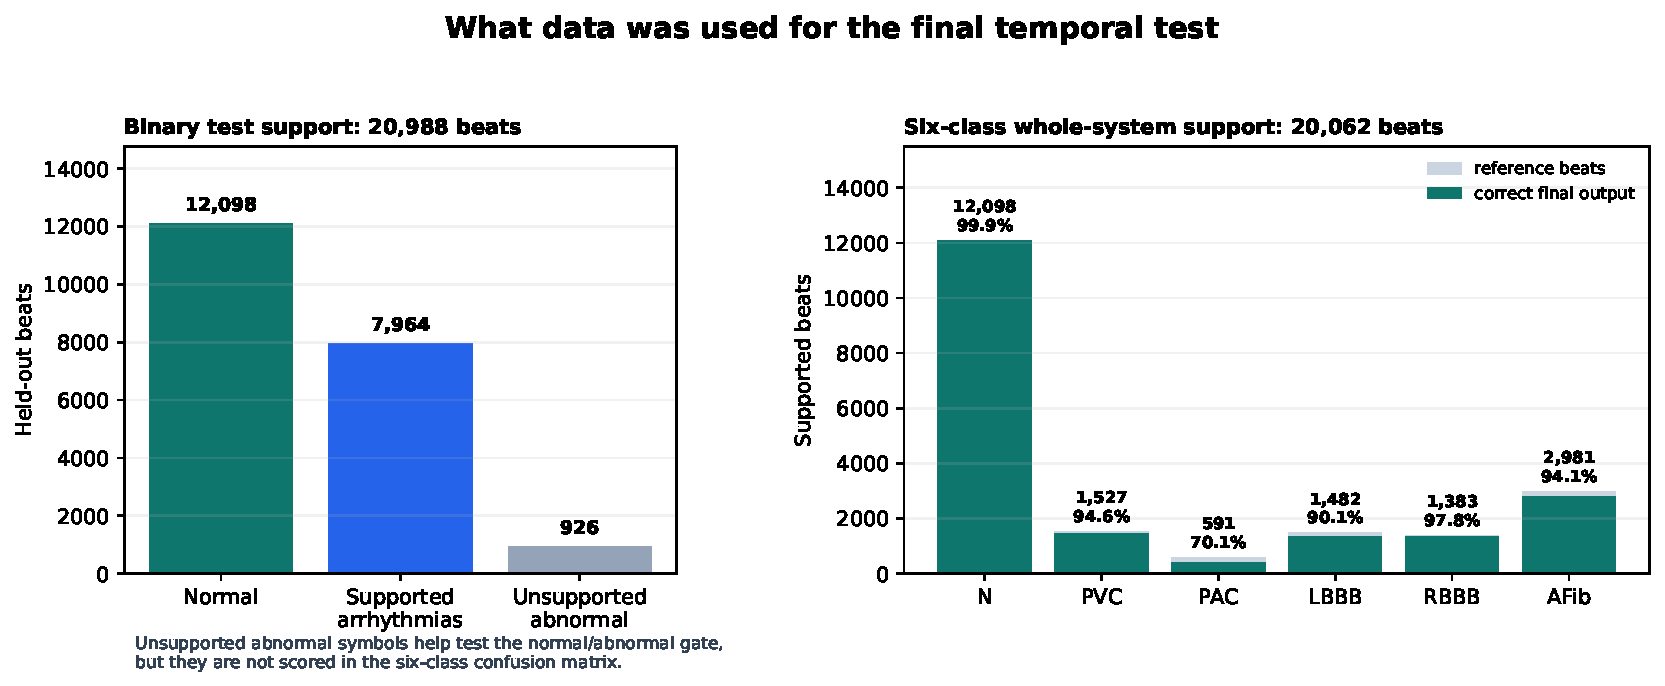
\includegraphics[width=.98\textwidth]{pic/generated/final_test_composition.pdf}
\caption{Reference-class composition of the corrected temporal test.}
\label{fig:final-test-composition}
\end{figure}

\section{Model selection}

Candidate selection uses the earlier 64--80\% region after the boundary
exclusions. The chosen binary model has 240 fully grown Extra Trees,
square-root feature sampling, minimum leaf size one, entropy criterion,
and subject/class weighting power 0.35. Its validation balanced accuracy is
98.73\%.
The chosen subtype model has 260 trees, feature sampling 0.33, minimum
leaf size one, entropy criterion, and weighting power 0.25. Its validation
macro F1 is 0.9811.

The binary threshold is 0.5708333333. The selected models are refitted on
83,050 development beats and 28,758 supported abnormal development beats,
respectively. The final test does not change this threshold.

\section{Main temporal results}

\begin{table}[H]
\centering
\caption{Corrected temporal results. Confidence intervals estimate
equal-subject accuracy, not pooled beat accuracy.}
\label{tab:final-headline}
\begin{tabular}{lrrrr}
\toprule
Outcome & Pooled & Subject mean & 95\% CI & Width\\
\midrule
Binary accuracy & 98.81\% & 98.84\% & 98.01--99.45\% & 1.44 pp\\
Conditional subtype & 97.63\% & 94.77\% & 89.03--99.08\% & 10.05 pp\\
Whole-system accuracy & 98.07\% & 98.03\% & 96.29--99.25\% & 2.95 pp\\
\bottomrule
\end{tabular}
\end{table}

In Table~\ref{tab:final-headline}, CI means confidence interval and pp means
percentage points. Interval widths are calculated from unrounded bounds;
subtracting the displayed bounds may therefore give a slightly different value.

Binary balanced accuracy is 98.69\%, sensitivity is 97.91\%, specificity is
99.47\%, precision is 99.27\%, and F1 is 0.9858. Conditional subtype macro
F1 is 0.9574; whole-system macro F1 is 0.9524.

\begin{figure}[H]
\centering
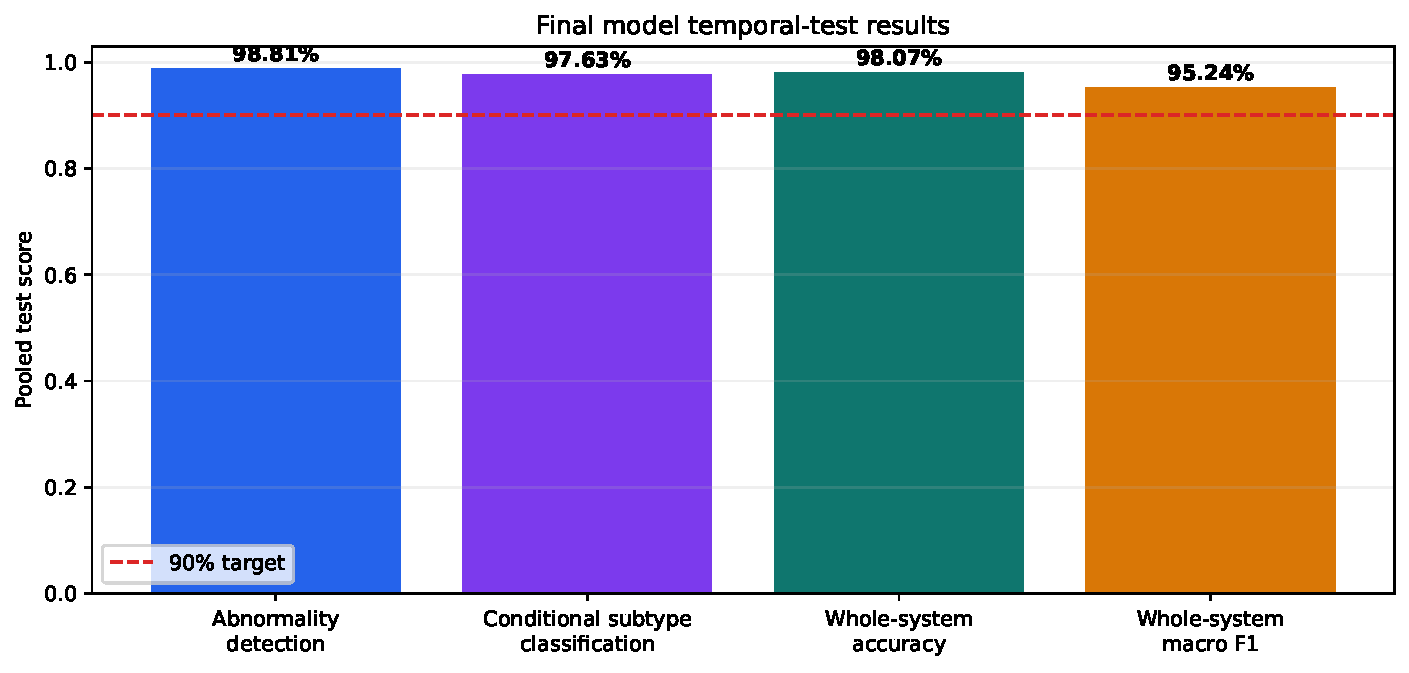
\includegraphics[width=.96\textwidth]{pic/generated/final_metrics.pdf}
\caption{Pooled temporal scores after the preprocessing correction.}
\label{fig:final-metrics}
\end{figure}

For the whole system, all three primary targets were met: pooled accuracy
was above 90\%, the lower confidence bound for equal-subject accuracy was
above 90\%, and interval width was at most three percentage points. These are descriptive outcomes of the
retrospective study. Prior test exposure prevents interpreting them as an
independent confirmation of these targets.

\section{Uncertainty and subject variation}

The bootstrap resamples 45 complete subject clusters with equal weight,
10,000 times using seed 20260801. It holds the fitted model fixed.
For subtype accuracy, subjects without supported abnormal test beats have
no subtype score and are omitted from that replicate's mean.

\begin{figure}[H]
\centering
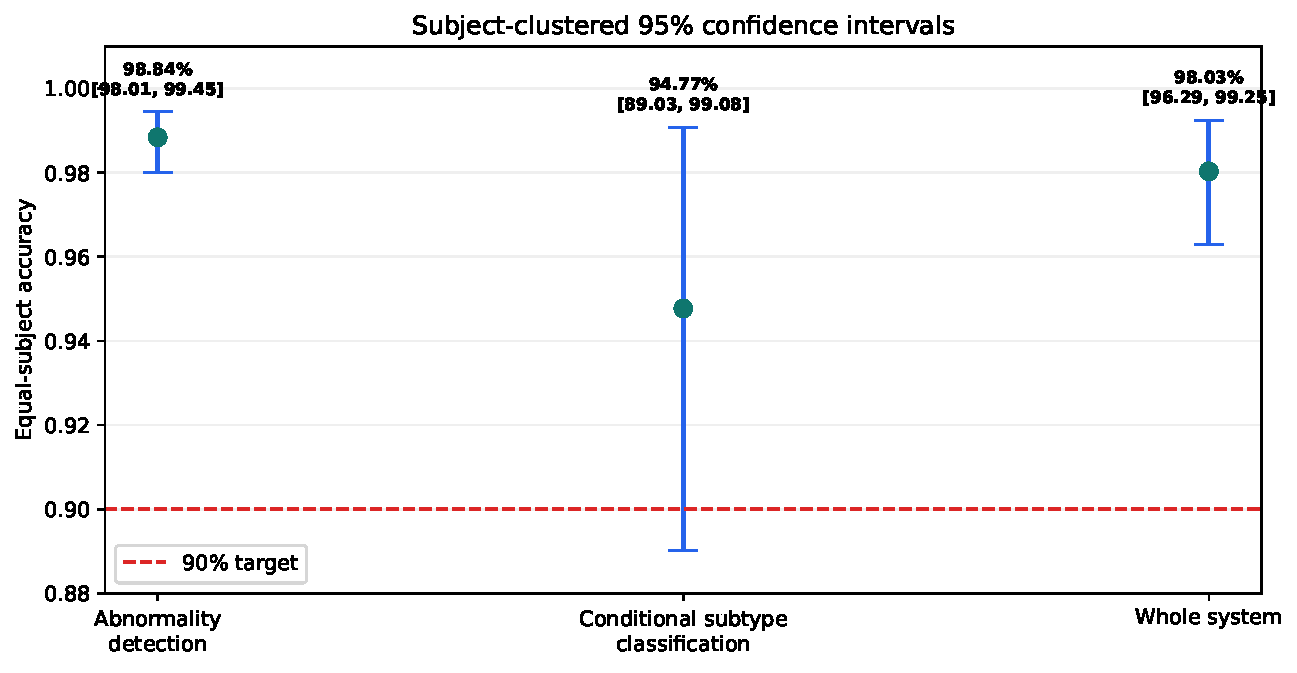
\includegraphics[width=.90\textwidth]{pic/generated/final_clustered_ci.pdf}
\caption[Subject-clustered confidence intervals.]{Equal-subject accuracy
and percentile bootstrap intervals. The conditional subtype interval remains
wide even though the whole-system width target is met.}
\label{fig:final-ci}
\end{figure}

Forty-three of 45 subject clusters exceed 90\% whole-system accuracy.
The exact one-sided sign test gives $p=2.94\times10^{-11}$ against the
null that no more than half of subjects exceed the target. The secondary
Wilcoxon statistic is 987, with $p=4.24\times10^{-8}$. Its location-shift
interpretation requires additional symmetry assumptions. Neither test
corrects selection optimism or establishes new-patient performance.

\begin{figure}[H]
\centering
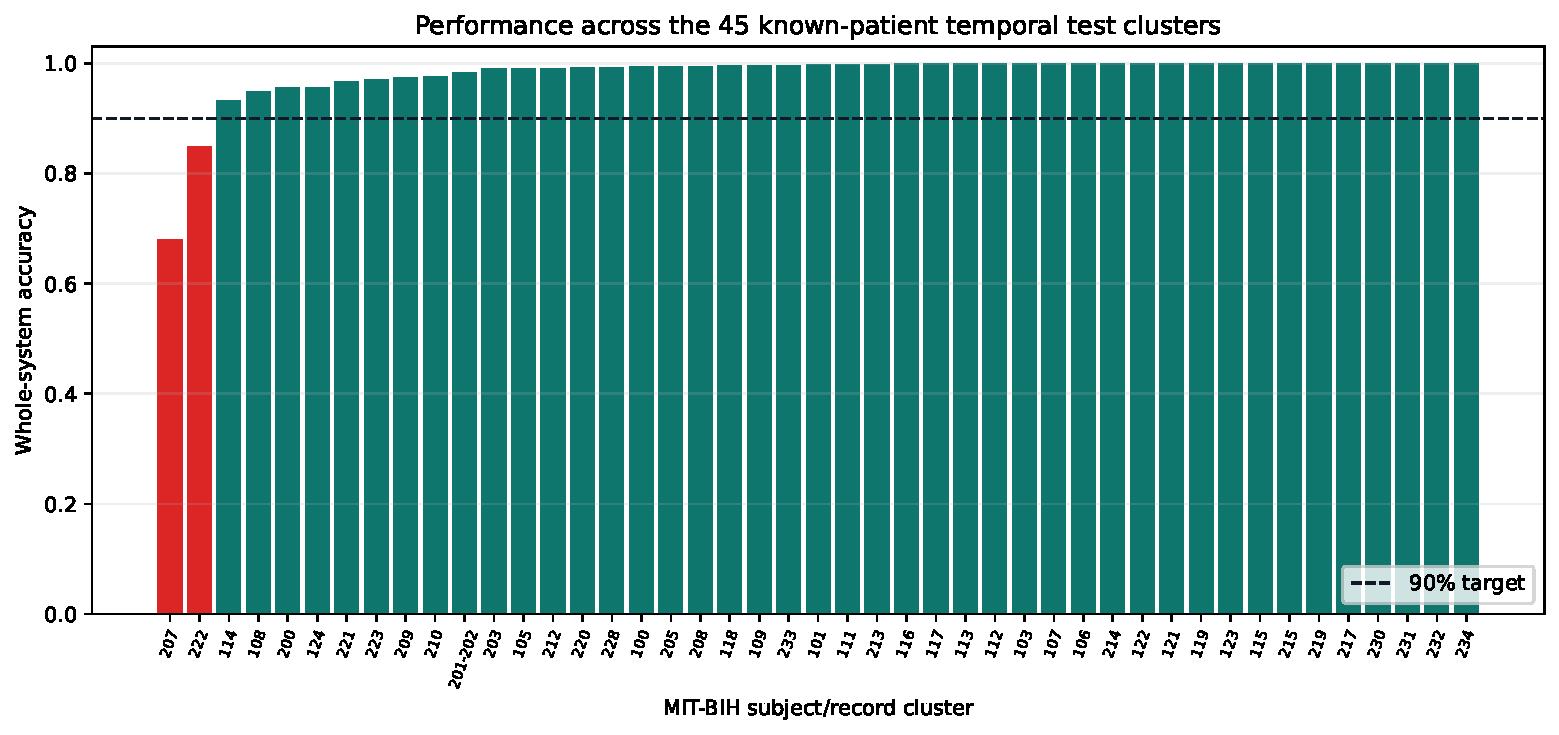
\includegraphics[width=.98\textwidth]{pic/generated/final_subject_accuracy.pdf}
\caption{Corrected whole-system accuracy across 45 known-patient clusters.}
\label{fig:final-subjects}
\end{figure}

The below-target clusters are 207 (67.92\%) and 222 (84.85\%). Cluster 207
has high binary accuracy but poorer subtype classification. Cluster 222 has
binary accuracy 85.45\%, so failures in the gate also matter. This variation
is not visible from pooled accuracy alone.

\section{Errors by stage and class}

The gate detects 8,698 of 8,884 abnormal beats and correctly assigns N to
12,021 of 12,085 N beats. Thus it produces 186 missed abnormal beats and
64 false alarms. When evaluated without the gate, the subtype model correctly classifies 7,769 of
7,958 supported abnormal beats. Gate errors can assign N to an abnormal beat even when the subtype model
would have classified it correctly.

\begin{table}[H]
\centering
\caption{Whole-system performance by supported abnormal output group.}
\label{tab:final-arrhythmias}
\begin{tabular}{lrrrrr}
\toprule
Group & True & Correct & Precision & Recall & F1\\
\midrule
PVC & 1,527 & 1,499 & 92.36\% & 98.17\% & 0.9517\\
PAC & 589 & 416 & 98.58\% & 70.63\% & 0.8229\\
LBBB & 1,481 & 1,476 & 96.72\% & 99.66\% & 0.9817\\
RBBB & 1,383 & 1,365 & 99.78\% & 98.70\% & 0.9924\\
AFib & 2,978 & 2,879 & 98.26\% & 96.68\% & 0.9746\\
\bottomrule
\end{tabular}
\end{table}

\begin{figure}[H]
\centering
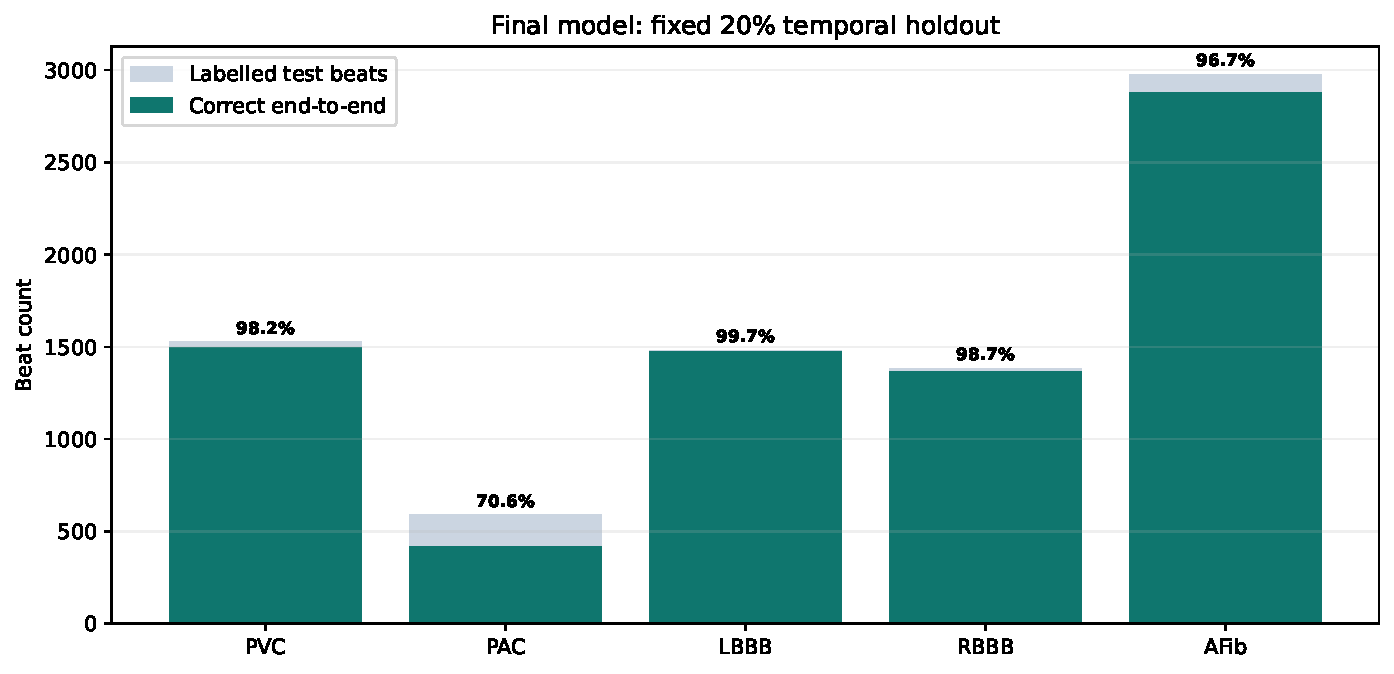
\includegraphics[width=.95\textwidth]{pic/generated/final_arrhythmia_counts.pdf}
\caption{True and correctly classified supported abnormal beats.
PAC remains below the 90\% recall target.}
\label{fig:final-arrhythmia-counts}
\end{figure}

Of 589 PAC-group beats, 549 pass the binary gate, 441 receive the correct
subtype when the gate is ignored, and 416 are correct end to end.
PAC errors therefore arise in both stages. AFib denotes the project's
AFIB/AFL rhythm grouping on normal-like beat symbols; the 96.68\% recall
is not an episode-level or AF-only sensitivity estimate.

\begin{figure}[H]
\centering
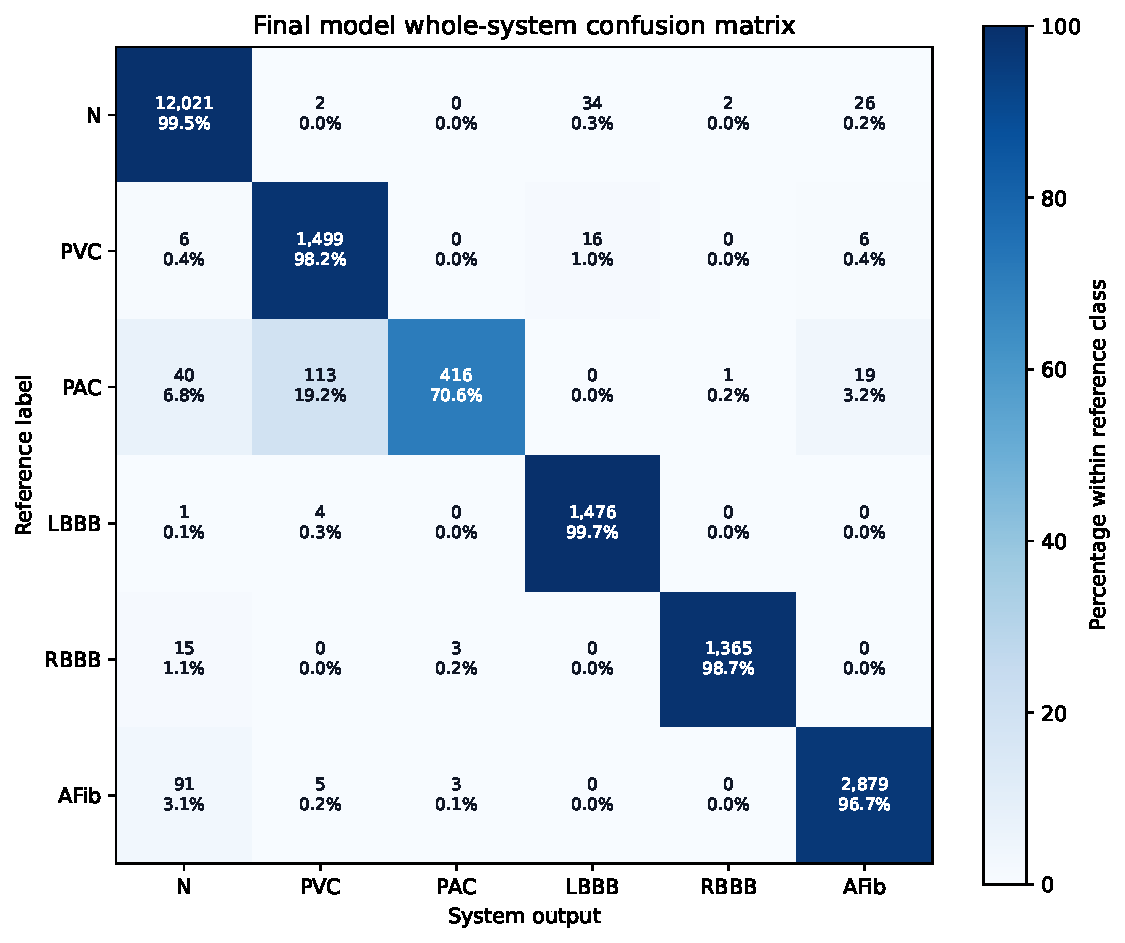
\includegraphics[width=.86\textwidth]{pic/generated/final_confusion_matrix.pdf}
\caption{Whole-system confusion matrix for 20,043 supported temporal beats.}
\label{fig:final-confusion}
\end{figure}

The largest abnormal-subtype confusion is 113 PAC beats assigned to PVC.
The gate sends 91 AFib-group and 40 PAC-group beats to N. Among reference N
beats, 34 become LBBB and 26 become AFib. Unsupported abnormal beats are
excluded from this matrix, but a deployed gated beat still receives a supported
subtype because the model has no unknown-class rejection rule.

\section{Limited external INCART check}\label{sec:external-incart}

The frozen hierarchy was evaluated on the limited INCART sample defined in
Section~\ref{sec:external-protocol}. The two records represent one source
patient and contain only N and PVC reference labels. Table~\ref{tab:external-incart-summary}
reports the measured performance on this sample.

\begin{table}[H]
\centering
\caption{Corrected model on complete INCART I01 and I02 recordings.}
\label{tab:external-incart-summary}
\begin{tabular}{lr}
\toprule
Quantity & Value\\
\midrule
Records / source patients & 2 / 1\\
Accepted annotated beats & 5,416\\
Reference N / PVC & 4,845 / 571\\
Fixed abnormal threshold & 0.5708333333\\
Binary accuracy & 94.11\%\\
Binary balanced accuracy & 96.55\%\\
Sensitivity / specificity & 99.65\% / 93.46\%\\
Binary precision / F1 & 64.22\% / 0.7811\\
AUROC / average precision & 0.9914 / 0.9152\\
TP / TN / FP / FN & 569 / 4,528 / 317 / 2\\
Whole-system accuracy & 92.85\%\\
End-to-end PVC recall & 87.74\%\\
\bottomrule
\end{tabular}
\end{table}

Only N and PVC occur in the reference labels. The binary model detects 569 of 571
PVC beats but produces 317 false alarms among 4,845 N beats. End to end,
501 PVC beats receive the correct label. Binary accuracies by record are
94.47\% for I01 and 93.74\% for I02. High binary sensitivity therefore
coexists with lower precision and subtype errors.

Macro F1 over the six predefined labels is 0.3039 when the four classes
absent from the reference labels are assigned F1 values of zero. The mean over the two observed reference
classes is 0.9116. These summaries are not directly comparable to a six-class
test containing reference examples of every class. PAC, LBBB, RBBB and AFib sensitivity cannot
be estimated from this subset. A patient-cluster population confidence
interval is not reported because there is only one source patient.


\section{Answers to the research questions}
\begin{description}
\item[RQ1] The frozen autoencoder supplies four residual features, but their
independent benefit has not been tested through a controlled comparison.
\item[RQ2] Binary, conditional-subtype and whole-system accuracies are
98.81\%, 97.63\% and 98.07\%, respectively, on their respective evaluation sets.
\item[RQ3] Equal-subject whole-system accuracy is 98.03\%, with a
96.29--99.25\% interval and two below-target subject clusters.
\item[RQ4] The whole-system targets were met, but PAC recall remained below
90\%. INCART evaluation covered only one patient and two reference classes;
broader external validation remains incomplete.
\end{description}
